\documentclass[12pt]{article}
\usepackage[paper=a4paper,left=30mm,right=30mm,top=35mm,bottom =35mm]{geometry}
\usepackage[utf8]{inputenc}
\usepackage[T1]{fontenc}
\usepackage{stmaryrd}
\usepackage{setspace}
\usepackage{mathrsfs}
\usepackage[ngerman]{babel}
\usepackage{amssymb}
\usepackage{amsmath}
\usepackage{fancyhdr}
\usepackage[dvips,unicode,colorlinks,linkcolor=black]{hyperref} 
\usepackage{graphicx}
\usepackage{float}

\pagestyle{fancy}
\lfoot{}
\rfoot{Paul Kremser, Tobias Grussenmeyer}
\cfoot{\thepage}
\fancyhead[L]{FPI Versuch: Rastertunnelmikroskop}
\renewcommand{\headrulewidth}{0.6pt}
\renewcommand{\footrulewidth}{0.6pt}
\setlength{\headheight}{16pt}
\setlength{\parindent}{0pt}
% Für die Wahl der Schriftart
\newcommand{\changefont}[3]{
\fontfamily{#1} \fontseries{#2} \fontshape{#3} \selectfont}

\begin{document}
% keine Hurenkinder und Schusterjungen
\clubpenalty = 10000
\widowpenalty = 10000 
\displaywidowpenalty = 10000

\onehalfspacing
% Schriftart
\changefont{ptm}{m}{n} 

\begin{titlepage}
\author{Paul Kremser, Tobias Grussenmeyer}
\title{Versuch: Rastertunnelmikroskop}
\date{Versuchsdurchführung: 19. und 26. November 2009} 
\maketitle
\thispagestyle{empty}
\end{titlepage}


\tableofcontents
\thispagestyle{empty}
\newpage
\pagenumbering{arabic}
\section{Überblick}
Bei der Rastertunnelmikroskopie wird eine Sonde, eine elektrisch leitende Nadel, meistens Spitze genannt über die Probe geführt. Der wechselwirkende Prozess ist der des quantenmechanischen Tunneleffekts. Bei einer angelegten Spannung zwischen einer Spitze und einer Oberfläche führt dies zu einem statisch messbaren Tunnelstrom. Der Tunnelstrom hängt vom Abstand zwischen Spitze und Probe ab. Durch Steuerung der Spitzte mittes Piezokristall lassen sich somit Höhenunterschiede in atomarer Größenordnung messen.

\section{Aufgabestellung}

\section{Theoretische Grundlagen}
Das Rastertunnelmikroskop bezeichnet den experimentellen Aufbau, in dem die Spitze zeilenweise über eine Oberfläche gerastert wird und der Tunnelstrom die zentrale Messgröße ist. Die Ortskoordinaten $(x,y)$ des Rasterfeldes sind ungeregelte Größen während der Tunnelstrom $I$ abhängig ist von der $z$-Position und der angelegten Spannung $U$ und meistens über eine Regelschleife miteinander verbunden ist. Die Abhängkeit voneinander bildet dabei verschiedene physikalische Eigenschaften der Oberfläche ab. $I(U)$ bei konstantem $z$ wird Tunnelspektroskopie genannt und $I(z)$ bei $U = const$ gibt Zugang zur Austrittsarbeit. Das Auftragen der Ortsabhängigkeit verschiedener Größen wird i.A. abbilden genannt. Dabei wird eine sehr hohe Auflösung bis zur atomaren Skala erzielt, da der dem RTM zu Grunde liegende Tunneleffekt sensitiv auf Änderungen im Sub-Angström-Bereich ist. Die Ortsabhängigkeit des Tunnelstroms spiegelt die Konvolution der realen Topographie mit elektronischen Eigenschaften wieder. Eine dreidimensionale Auftragung suggeriert dabei einen pseudomäßigen Blick auf die Oberflächentopographie bildet aber exakterweise die Höhentopologie konstanter Elektronendichte ab.

\section{Versuchsaufbau}
\begin{figure}[H]
\centering
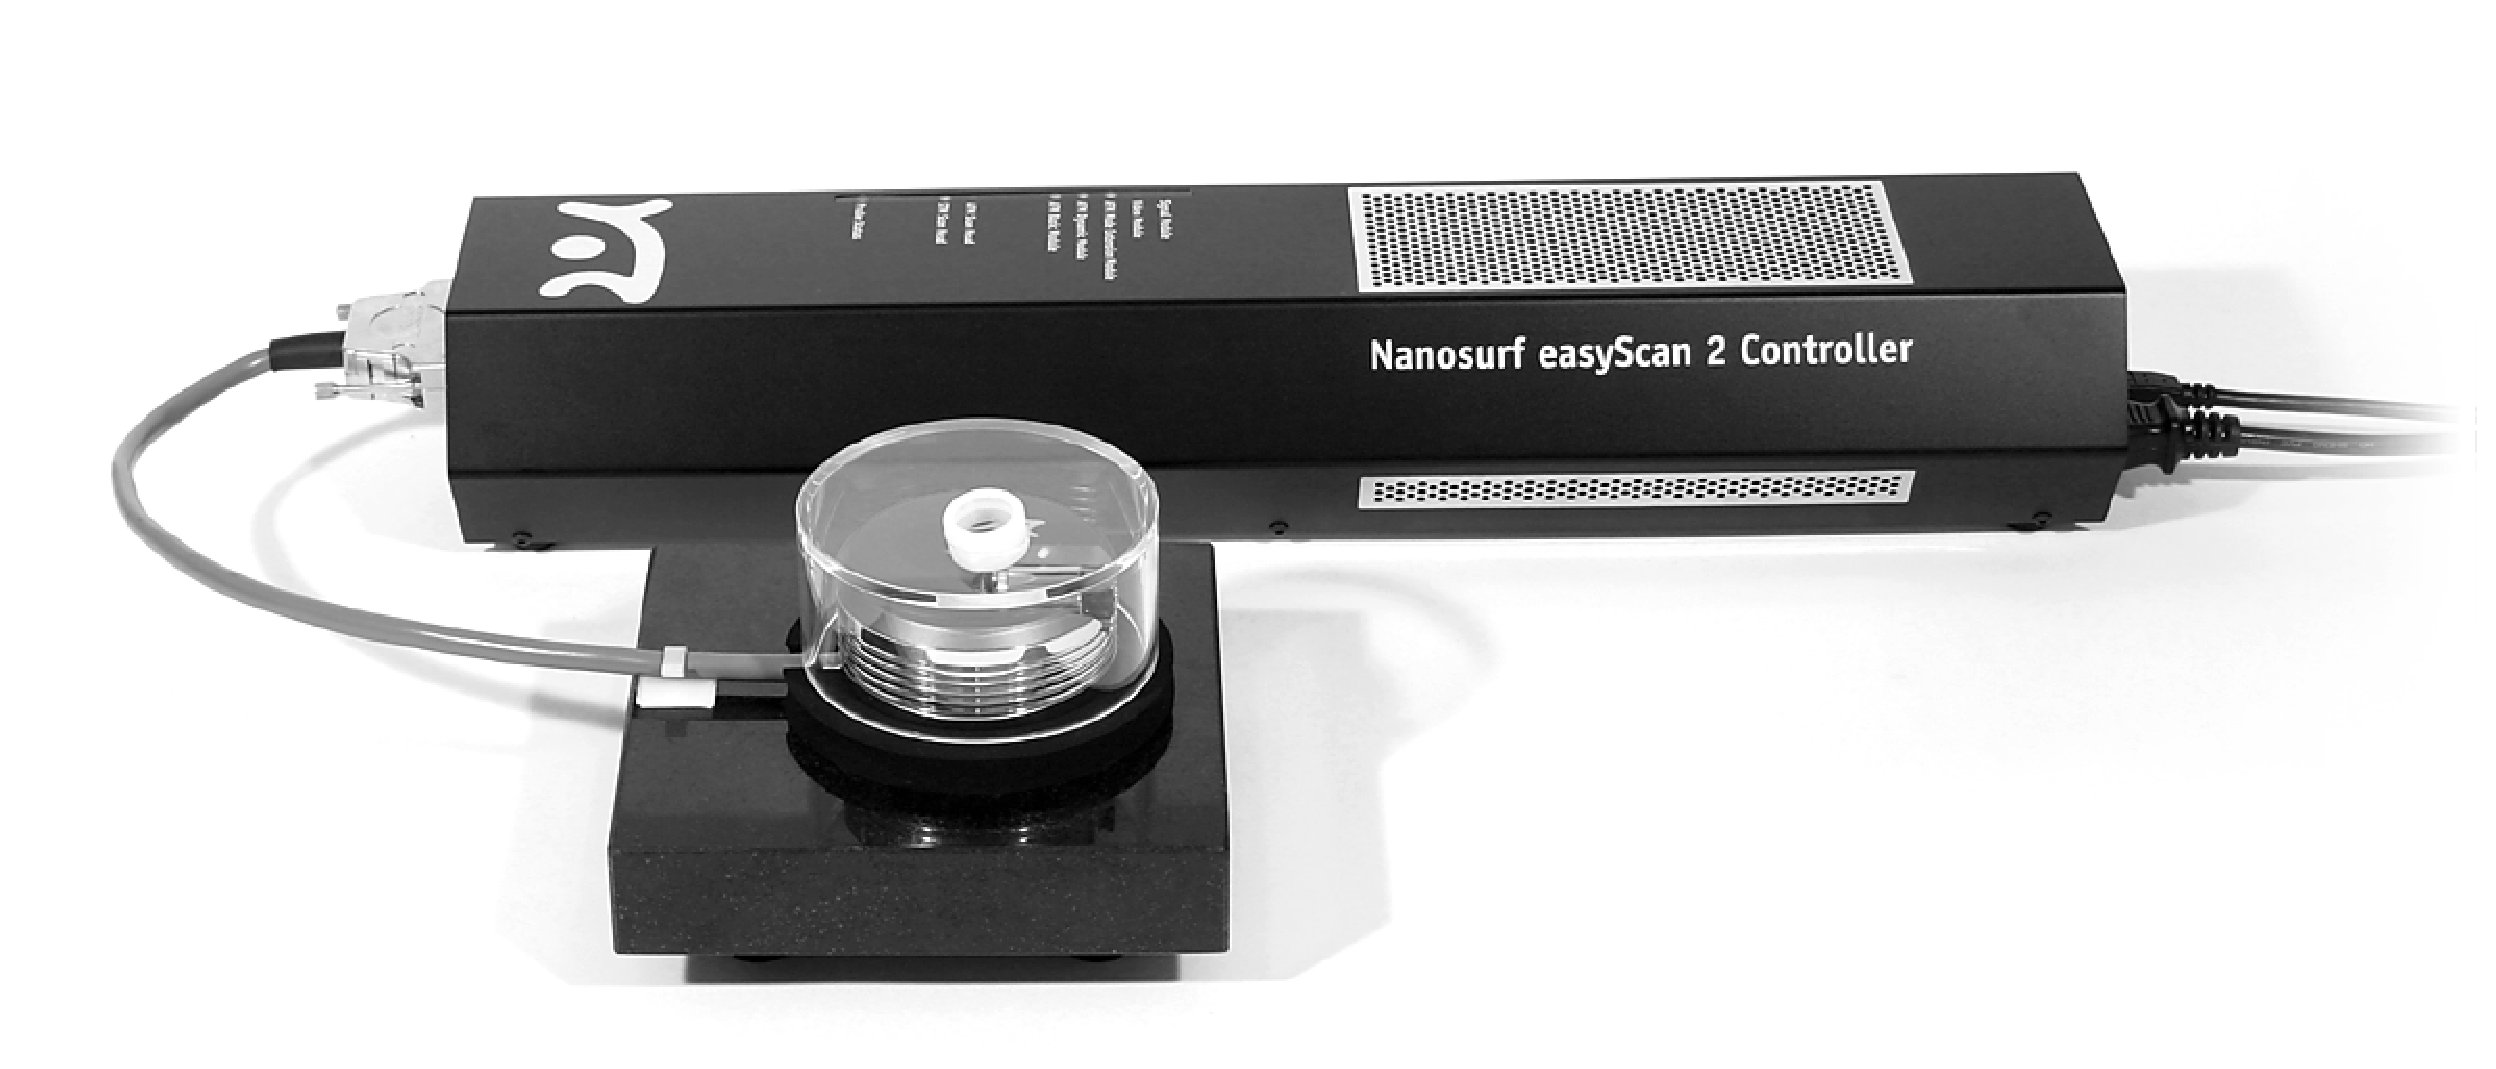
\includegraphics[width=0.9\linewidth]{pictures/aufbau.eps}
\caption{Das RTM mit Steuereinheit}
\end{figure}

\begin{figure}[H]
\centering
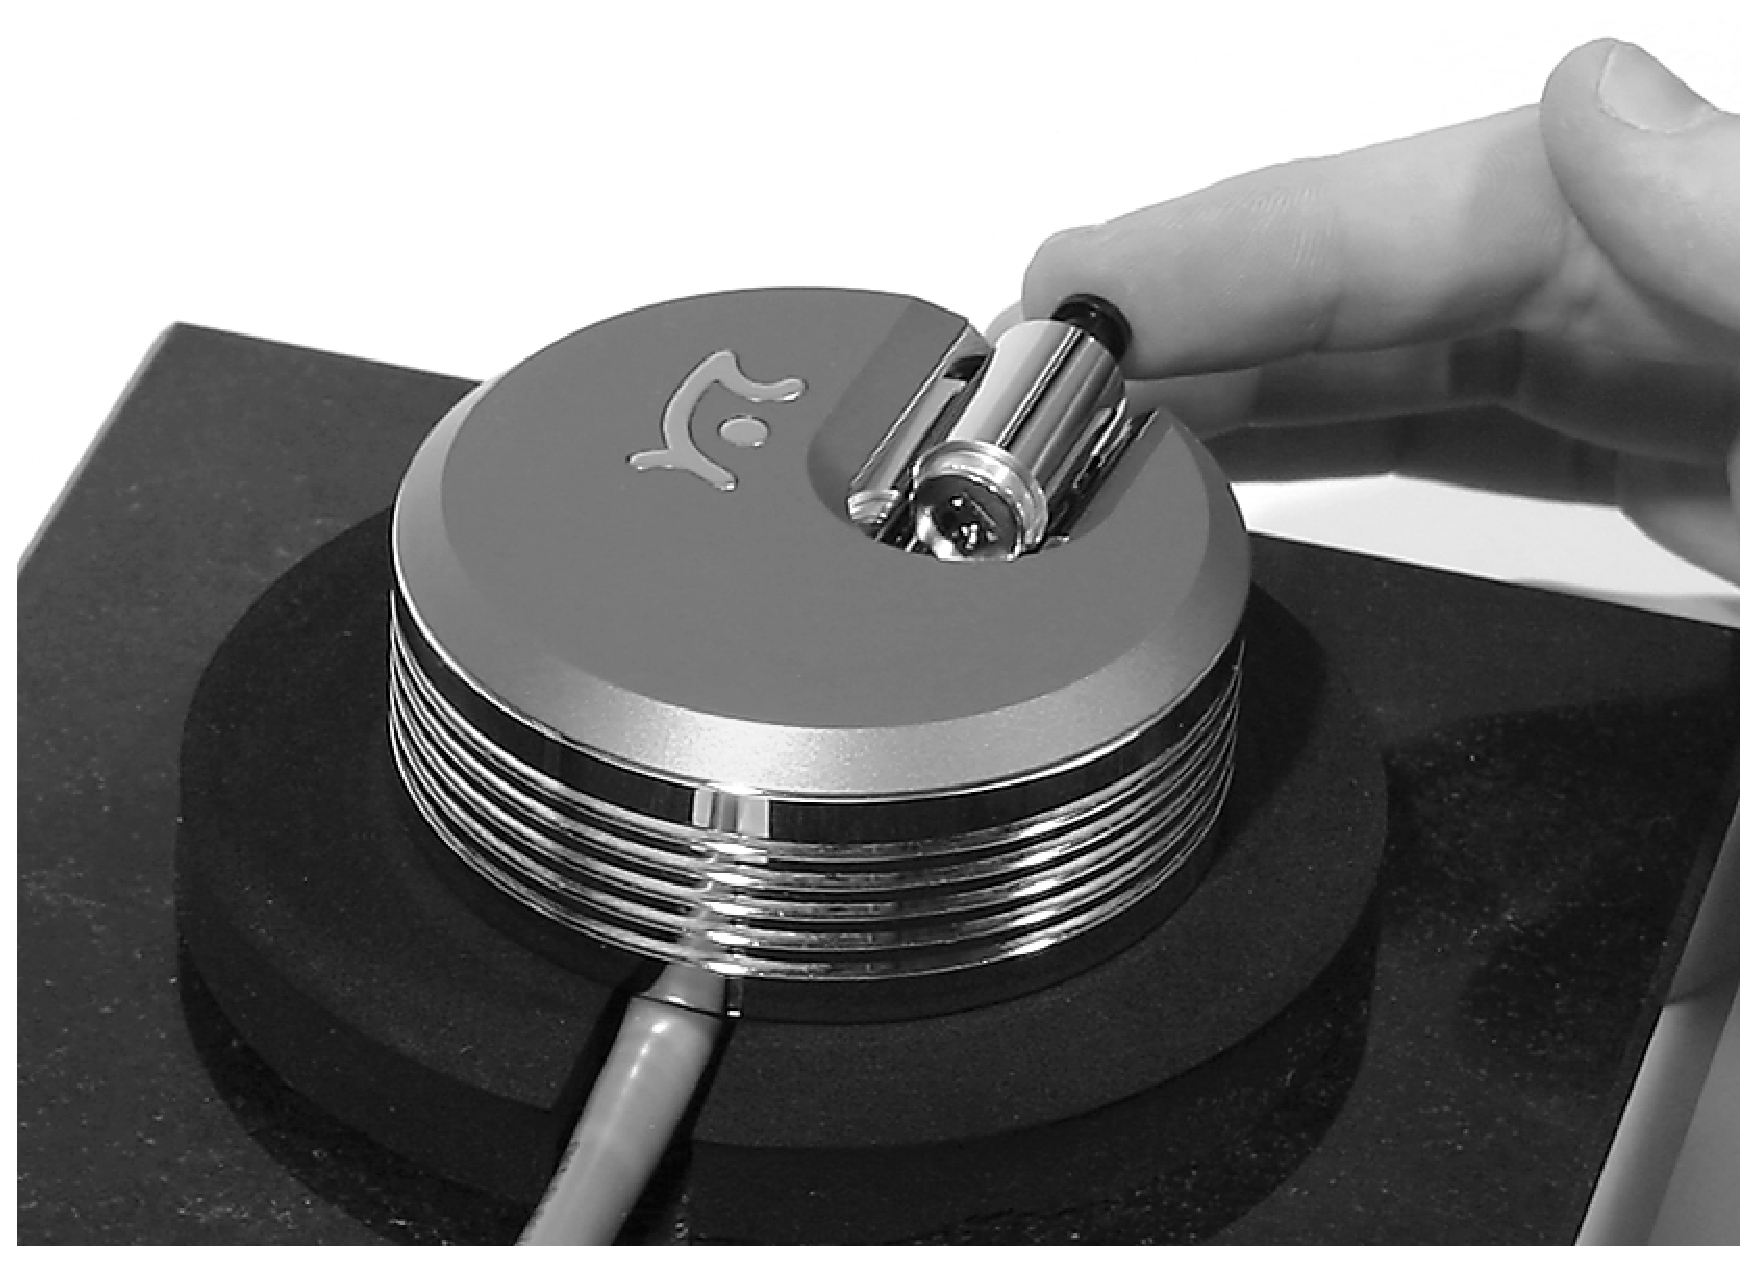
\includegraphics[width=0.9\linewidth]{pictures/rastertunnel.eps}
\caption{Das eigentliche RTM}
\end{figure}
\section{Durchführung}
Zu Beginn, wie auch noch mehrmals während des Versuchs muss eine Spitze hergestellt werden. Hierzu wird mit einem Seitenschneider ein Platin-Iridium-Draht angeschnitten und dann abgerissen. Die Spitze und Probe werden in das Mikroskop eingesetzt. Die Probe befindet sich auf einem Probenhalter welcher als Schlitten elektronisch gesteuert werden kann. Anfangs wird die Probe von Hand auf ca. $1mm$ Abstand zur Spitze gebracht und dann mittels der Elektronik weiter an die Probe angenähert.
Bei dem automatisierten Annäherungsprozess kam es oft vor das die Probe gegen die Spitze stieß und die Spitze ausgewechselt werden musste. \\

Unter verwendung etlicher Spitzen haben wir schlussendlich die drei Proben vermessen.
\section{Auswertung}
\begin{figure}[H]
\centering
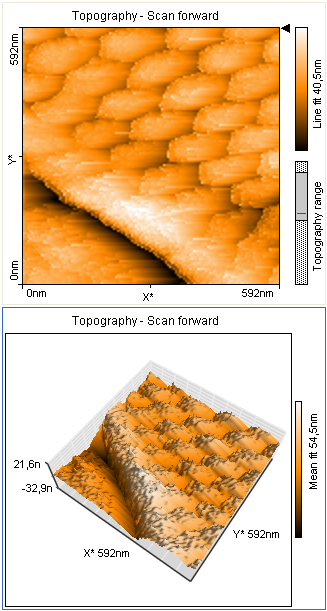
\includegraphics[width=0.9\linewidth]{../plot/data/goldgitter/goldgitter.PNG}
\caption{Goldgitter}
\end{figure}
\section{Zusammenfassung}

\end{document}
